% !TEX engine = xelatex
\documentclass[10pt,oneside,letterpaper,landscape]{memoir}

% set your margins here; left margin, right margin, bottom margin, top margin, binding offset, etc
\usepackage[lmargin=13mm,rmargin=13mm,bmargin=11mm,tmargin=13mm,bindingoffset=0mm,heightrounded]{geometry}

% these are used for placing text outside the natural flow of text, in blocks and boxes (and even rotated)
\usepackage[absolute]{textpos}
\setlength{\TPHorizModule}{10mm}
\setlength{\TPVertModule}{10mm}
\usepackage{rotating}

% this allows you to use images
\usepackage{graphicx}
\graphicspath{ {images/} }

% font stuff
\usepackage{fontspec,xltxtra,xunicode}
\defaultfontfeatures{Mapping=tex-text}

% main font, used for the full document; use the family name here. If scale = 1 it is 10pt; you may want to go to .9 or even .8
\setmainfont[Ligatures=TeX,Scale=1]{Times New Roman}

% each of these is a font we'll use later; you can add more and scale them using the same method
% you may want more or less of these; at minimum, you want a title font and a section header font
% you'll need to mess with scale on these to get them looking 'nice' for your fonts
\newfontfamily\titlefont[Ligatures=TeX,Scale=2.5]{Courier}
\newfontfamily\sectionfont[Ligatures=TeX,Scale=1]{Arial}

% this is for the purposes of Lettrine
\newfontfamily\numeralfont[Ligatures=TeX,Scale=1]{Courier}

% new commands; these allow us to set up references to our fonts and format them in advance
\newcommand*\toptitle[1]{{\color{titlecolor}\titlefont{#1}}}
\newcommand*\tagline[1]{{\color{taglinecolor}\taglinefont{#1}}}

% this is a seperator, like a dagger or bullet, for inline lists
\newcommand*\sep[0]{\* }

% this lets us use multiple columns
\usepackage{multicol}
% this sets how much space between any two columns
\setlength{\columnsep}{2em}

% this is for tables
\usepackage{tabularx}

% and here's where we define colors, giving each a name so we can refer to it
\usepackage{xcolor}

% first basic stuff 
\definecolor{offwhite}{HTML}{ffffff}

% now single use case items like 'text I put in the margins'
\definecolor{margintext}{HTML}{363b4d}

% ... and box corners/backgrounds
\definecolor{plainboxbg}{HTML}{F3F3F3}
\definecolor{plainboxtxt}{HTML}{000000}
\definecolor{plainboxtabs}{HTML}{363b4d}

% ... and the title color
\definecolor{titlecolor}{HTML}{363b4d}
\definecolor{taglinecolor}{HTML}{363b4d}

% ... and section header color
\definecolor{shadecolor}{HTML}{909090}

% this is just a convenience function to put a box around text
\newcommand{\shadebox}[1]{\par\noindent\colorbox{shadecolor}
{\parbox{\dimexpr\textwidth-2\fboxsep\relax}{#1}}\smallskip}

% this puts a repeating symbol over and over to the left of the text; an alternate header
\newcommand\rep{\leavevmode\xleaders\hbox{.}\hfill\kern0pt}

% this creates fancier boxes
\usepackage[raster, skins, hooks, many]{tcolorbox}

% ... but we're just creating a simple one to start
\newtcolorbox{plainbox}[1][]{fonttitle=\color{white}\headfont, colframe=shadecolor, colback=white, after skip=2mm, #1}

% drop caps, very useful for mechanic results
\usepackage{lettrine}
\renewcommand{\LettrineFontHook}{\numeralfont}
\setlength{\DefaultNindent}{2pt}
\setlength{\DefaultFindent}{2pt}

% uncomment this to change the entire page's background
%\pagecolor{\color{50!red}}

% hide links so they're not marked out
\usepackage[hidelinks]{hyperref}

% and now some general formatting; you can adjust other parts by changing 'sec' to 'subsec' or 'subsubsec'

% remove numbering from section titles, as we'll use our sections as dividers between rules chunks
\setsecnumformat{}

% now reduce spacing around section tags
\setaftersecskip{1mm}
\setbeforesecskip{3mm}

% and redefine what font we use for section heads
\setsecheadstyle{\sectionfont\color{blue}}% Set \section style

% save the current indent so you can use \indent when you want to indent
\newlength\tindent
\setlength{\tindent}{\parindent}
\renewcommand{\indent}{\hspace*{\tindent}}

% and here we set the default indent to nothing and a line between paragraphs instead
\setlength{\parindent}{0pt}
\setlength{\parskip}{.5\baselineskip}

% make it so text doesn't squash down to the bottom
\raggedbottom

% now remove page numbering since this is just one sheet
\pagestyle{empty}

% this redefines minipage (basically an invisible box) to use all the same settings as above
\newlength{\currentparskip}
    \newenvironment{mpage}[1]{%
        \setlength{\currentparskip}{\parskip}% save the value
             \begin{minipage}{#1}% open the minipage
         \setlength{\parskip}{\currentparskip}% restore the value
    }
{\end{minipage}}

% and this sets up a double rule you can use as a divider
\newcommand{\doublerule}[1][.4pt]{%
  \noindent\color{black!75}
  \makebox[0pt][l]{\rule[.7ex]{\linewidth}{#1}}%
  \rule[.3ex]{\linewidth}{#1}\color{black}\vspace{-1mm}}

  % and finally, just some dummy text
  \usepackage{blindtext}

%%% BEGIN DOCUMENT; this is required
\begin{document}

% set up 3 columns; this will be matched at the very end with \end{multicols}
\begin{multicols}{3}

%  I like to set up any textblocks (from textpos package) up front. The 13 is how wide the textblock is, and the 13.5 and 21 tell you how high on the page and how far over it is. Try setting it to 0,0 to see the difference.
  \begin{textblock}{15}(19,21)
      \footnotesize
      	\textit{\href{https://www.flickr.com/photos/79023099@N00/5506704850}{"Godzilla Guitar Hero"}} by \textit{\href{https://www.flickr.com/photos/79023099@N00}{Wild Guru Larry}} is licensed under \textit{\href{https://creativecommons.org/licenses/by/2.0/?ref=ccsearch&atype=rich}{CC BY 2.0}}.
  \end{textblock}

% this is how you add another textblock, and how you include a graphic
\begin{textblock}{18}(18.25,6.25)
    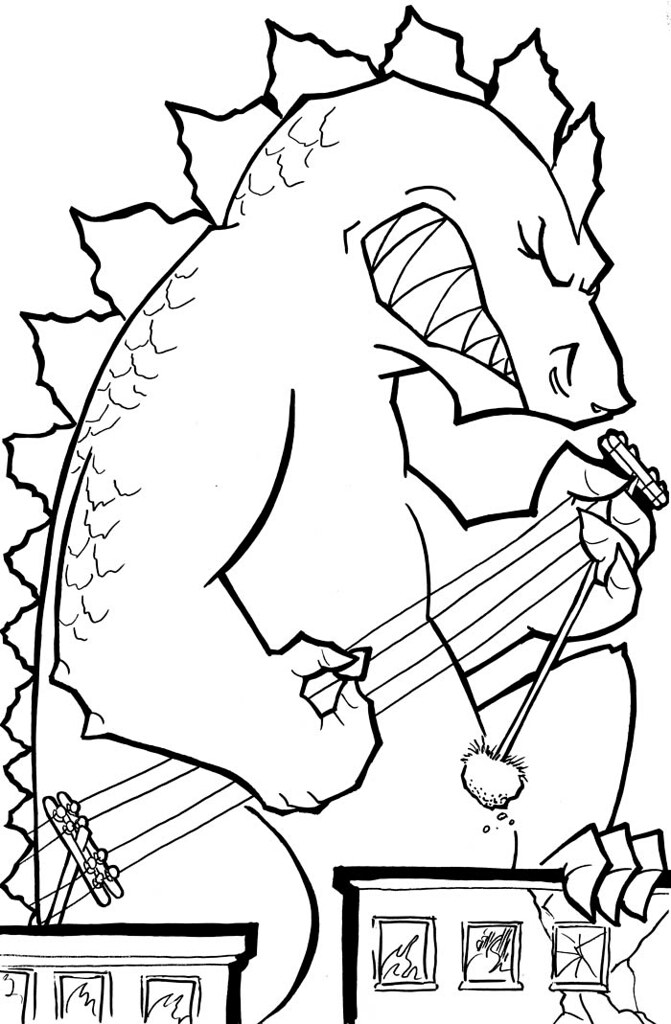
\includegraphics[width=.5\textwidth]{images/5506704850_a8cce4bb2c_b.jpg}
\end{textblock}

% now we start laying it out

%vspace and hspace adjust the vertical space above their line and the horizontal space before it, respectively
% the asterisk says 'no really, do this' if latex for some reason won't

% first, open a mpage, our custom minipage

% columnwidth is the width of one column, in this case, a third of the page. By putting a number in front of it, you can multiply it by that number 
% two columns is roughly 2.13. This stretches the invisible block across two columns.
\begin{mpage}{2.13\columnwidth}

 \hspace*{0mm}{\toptitle{Legally Distinct Kaiju RPG}}

% a little extra space over what'd normally be provided
\vspace{3mm}

\textit{A game about giant monsters terrorizing the city, by} \textit{\href{https://astralfrontier.itch.io}{Astral Frontier}}

\doublerule

\end{mpage}

% a little extra space over what'd normally be provided
\vspace{2mm}

\section{Character Creation \rep}

One player is the Kid. They narrate for themselves, the monster, and all NPCs.

All other players create a character from one of three factions: Civilian, Scientist, or Military.

Everything the Kid says in-character about the monster is true. Nobody else knows this at first.

Determine at least one B-plot before play begins. Every player involved in a B-plot must approve of it.

\subsection{Example Characters}

Create your own, choose from this list, or roll 1d6:
\begin{enumerate}
	\item The intrepid reporter
	\item The ordinary blue-collar worker
	\item The old-coot science expert
	\item The plucky science assistant
	\item The grizzled four-star general
	\item The brave soldier
\end{enumerate}

\subsection{Example B-Plots}

Create your own, choose from this list, or roll 1d6:
\begin{enumerate}
	\item International tension
	\item Someone stole something
	\item Reporters or spies on the trail of something
	\item Construction of a power plant, road, etc. is threatened by the monster's presence
	\item Romance or rivalry between characters
	\item Aliens are invading or infiltrating Earth
\end{enumerate}

\vfill\null % if the text isn't compressed enough, use this to "fill" the rest of the column

\columnbreak

% now we put in some vertical space, which depends on your font and title, to account for the overlapping minipage. Note the dot.
{\color{white}.}
\vspace{18mm}

\section{Playing the Game \rep}

The monster starts the game with 3 HP.

The Kid narrates the current threat of the monster, while other players narrate the reactions from themselves or their faction as a whole.

\textbf{When anyone hatches a plan to defeat the monster}, describe it and roll 1d6.

If you spent a scene advancing any B-plot, or introduced drama to an existing plot, add +1d6 to the roll per distinct contribution. If anyone hammed it up, add +1d6 per ham.

Look for the highest roll on any of the dice.

\begin{enumerate}
	\item [1-3:] It fails. A player from another faction (e.g. Scientist when a Military player rolled) must come up with an explanation of why.
	\item [4-5:] The monster develops a new bullshit power, nullifying the plan. Any player can make suggestions, with the Kid's player having the final say.
	\item [6:] Mark 1 HP off the monster. The player who rolled describes the outcome.
\end{enumerate}

\subsection{Examples of Hamming It Up}

A Civilian interfered with the plan for some selfish or venal motive.
A Scientist horribly mangles real-world science.
The Military brags about the power of their new weapons.
The Kid is allowed to run wild through an off-limits area.

\subsection{Safety Check}

This is a game about giant monsters terrorizing cities. Everyone has their own ideas about what this means, including the original filmmakers. If the game isn't fun for you because of the material or the other players, speak up. If someone speaks up, stop and listen. Everyone's fun and comfort matters more than finishing the game.

\columnbreak

\section{Finishing the Game \rep}

Once the monster is at 0 HP, it is killed, driven off, etc. Resolve any lingering B-plots. If there is a sequel:

\begin{itemize}
\item A different player becomes the Kid
\item The monster returns from its defeat, but is now on the side of humanity
\item Devise a new threat for this monster to fight
\end{itemize}

% this ends our multicols
\end{multicols}

% this ends our document
\end{document}
